\section {Assignment 4 \\ {Salt and Pepper Noise}}
\label {sec:assignment_4}

\subsection{Manipulate own image from assignment 2}

In this assignment, a program was used to darken the image and add RGB salt and pepper noise to our original image from assignment 2. The noise must be filtered out and the brightness must be corrected.

We implemented a median filter and a gamma correction function to filter our image. The result is shown in figure \ref{fig:fortGT_Noise}.

\begin{figure}[h!]
    \centering
    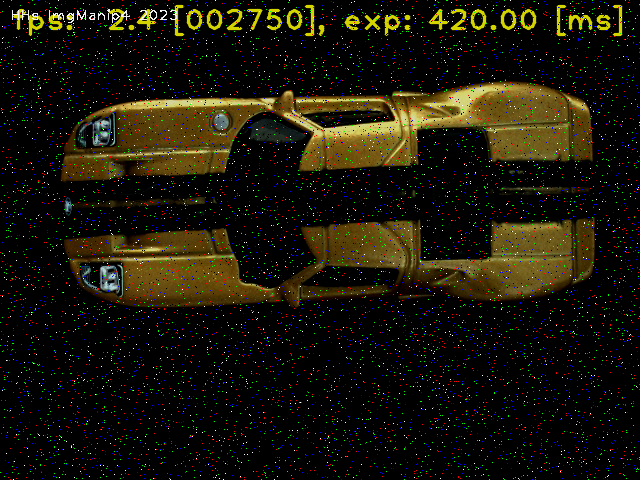
\includegraphics[width=0.45\textwidth]{fortGT_Noise.png}
    \caption{Image with salt and pepper noise}
    \label{fig:fortGT_Noise}
\end{figure}

\subsection{Write C/C++ code for Brightness correction}

A Brightness correction filter was written and can be found in appendix \ref{sec:appendix_B}. The filter function is shown in listing \ref{lst:brightness_correction}.

\begin{lstlisting}[language=C, caption={Brightness correction}, label=lst:brightness_correction]

void gammaCorrection(Mat* input, Mat* output, float gamma) {
    Size s = input->size();
    long h, w;
    float sum;
    
    std::cout << "Correcting gamma" << std::endl;
    uint8_t out[s.height][s.width];
    uint8_t lut[256];	
    
    for (int i = 0; i < 256; i++) { //create a lookup table, with the gamma correction curve.
        lut[i] = saturate_cast<uint8_t>(pow((float)(i / 255.0), gamma) * 255.0f); //saturate cast negative values to 0, and higher values to 255 (uint8_t or unsigned char)
        //std::cout << unsigned(lut[i]) << " "; //print the function for testing. cout prints uint8_t as chars so we cast it.
    }
    
    
    for (w=0; w<s.width; w++){ //loop over the image, 
        for(h=0; h<s.height; h++){
            sum = lut[(input->at<uint8_t>(h,w))]; //the original output value will be scaled to the value in the LUT.
            out[h][w]=(uint8_t)sum;
        }
    }
    std::memcpy(output->data, out, s.height*s.width*sizeof(uint8_t)); //copy our standard 2D array to a new buffer that OpenCV understands
}
\end{lstlisting}

We had several options for correcting brightness. At first we considered simply increasing the value of each pixel by addition. However, this would significantly increase the brightness of the black background turning it dark grey. For this reason we settled on using a gamma correction curve instead. This would spread the histogram "bins" rather than moving them up. Determining the correct gamma correction constant was trial and error, exponents below 0,5 would make the object too bright. 

\subsection{Write C/C++ code for ‘Salt and Pepper Noise’ correction}

A ‘Salt and Pepper Noise’ correction filter was written and can be found in appendix \ref{sec:appendix_B}. The filter function is shown in listing \ref{lst:noise_filter}.

\begin{lstlisting}[language=C, caption=Noise correction filter, label=lst:noise_filter]
void filter(Mat* input, Mat* result) {
    Size s = input->size();
    long h, w;
    long sum;
    
    //std::cout << "Input type was : " << input->type() << std::endl;
    uint8_t out[s.height][s.width];
    
    std::cout << s.height << " " << s.width << std::endl;
    
    for (w=0; w<s.width; w++){ //loop over the image, 
        for(h=0; h<s.height; h++){
            sum = 0;
            std::vector<uint8_t> median;
            
            for (int _x = -1; _x < 2; ++_x) //for every pixel, loop over every pixel in a 3x3 kernel
            {
                for (int _y = -1; _y < 2; ++_y)
                {
                    int idx_y = h + _y; //sum the incrementor with the kernel's, so we can identify borders
                    int idx_x = w + _x;
                    
                    if (idx_x < 0 || idx_x > s.width) //the kernel goes outside of the image, therefore break and ignore that pixel.
                        break;
                        
                    if (idx_y < 0 || idx_y > s.height)
                        break;
                    
                    median.push_back(input->at<uint8_t>(idx_y,idx_x)); // Add all the pixels from the kernel into a vector
                }
            }
            std::sort(std::begin(median), std::end(median)); //sort all pixel values from high to low
                    
            for (auto it = median.begin(); it != median.end(); ++it) {
                sum = median.at(median.size()/2); //The pixel at the y,x coordinate is now the median from our 3x3 sliding window
            }
            out[h][w]=(uint8_t)sum;
        }
    }
    // this did not work, since the out array was never copied to memory, causing image data pointing to nowhere!
    //result = Mat(s.height, s.width, CV_8U, out); 
    // Instead, the data from out needs to be copied directly to Mat result with the correct size
    std::memcpy(result->data, out, s.height*s.width*sizeof(uint8_t));
}

\end{lstlisting}

The reason why we chose to implement a median filter is to preserve sharp edges to minimize loss of detail on the object, whereas a Gaussian or mean filter would blur sharp edges. In our code, a 3x3 sliding window is ran over the image, and the center pixel is replaced with the median of the window. The pixel values from the kernel are pushed back into a std::vector, this allows us to use STL library operations like std::sort to order the values.
After applying the median filter, the resulting image looks slightly blurred, but sharp transitions are mostly preserved. Note that the 1px wide text at the top of the image is partially removed. This is due to the nature of a median filter and is very challanging to preserve.

The result after applying the noise removal filter is snow below \ref{fig:fortGT_Noise_Filtered}.
\begin{figure}[h!]
    \centering
    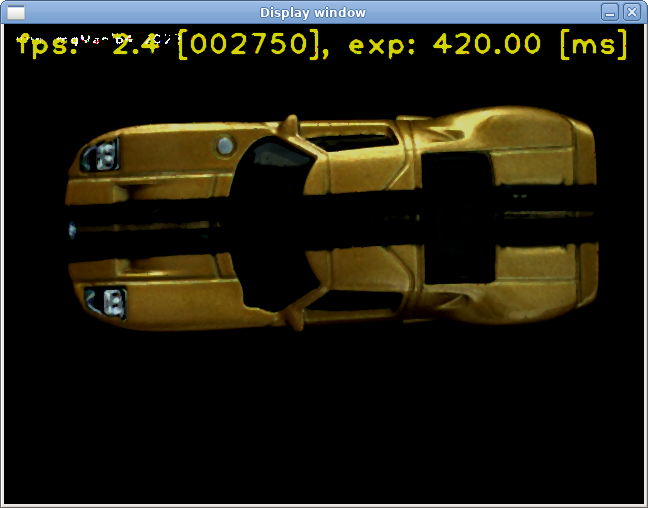
\includegraphics[width=0.45\textwidth]{fortGT_Noise_Filtered.png}
    \caption{Filtered image}
    \label{fig:fortGT_Noise_Filtered}
\end{figure}

The final result is shown in the figure below \ref{fig:fortGT_Filtered_corrected_05}. We chose a gamma correction factor of 0.5 but other values can also be used.
\begin{figure}[h!]
    \centering
    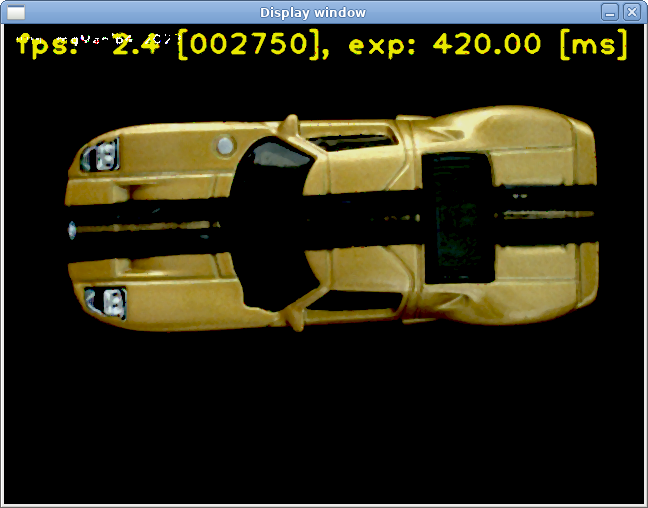
\includegraphics[width=0.45\textwidth]{fortGT_Filtered_corrected_05.png}
    \caption{Gamma correction on the filtered image}
    \label{fig:fortGT_Filtered_corrected_05}
\end{figure}
